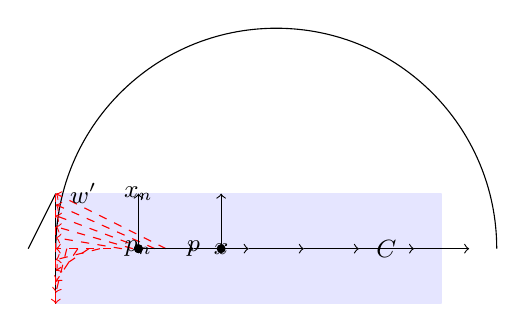
\begin{tikzpicture}[scale=0.7]
	\tikzstyle{every node}=[font=\small]
	\shade[left color=blue!10,right color=blue!10] (-3,1)--(4,1)--(4,-1)--(-3,-1)--cycle;
	\draw (-3,0) arc (180:0:4);
	\draw (-3,-1)--(-3,1);
	\draw (-3,1)--(-3.5,0);
	\draw[dashed,->,red] (-3,1)--(-3,-1);
	\draw[dashed,->,red] (-2.8,0)--(-3,-0.8);
	\draw[dashed,->,red] (-2.6,0)--(-3,-0.6);
	\draw[dashed,->,red] (-2.4,0)--(-3,-0.4);
	\draw[dashed,->,red] (-2.2,0)--(-3,-0.2);
	\draw[dashed,->,red] (-2,0)--(-3,0);
	\draw[dashed,->,red] (-1.8,0)--(-3,0.2);
	\draw[dashed,->,red] (-1.6,0)--(-3,0.4);
	\draw[dashed,->,red] (-1.4,0)--(-3,0.6);
	\draw[dashed,->,red] (-1.2,0)--(-3,0.8);
	\draw[dashed,->,red] (-1,0)--(-3,1);
	\node at (-2.5,1) {$w'$};
	\node at (-1.5,0) {$p_{n}$};
	\draw[->] (-1.5,0)--(-0.5,0);
	\draw[->] (-0.5,0)--(0.5,0);
	\draw[->] (0.5,0)--(1.5,0);
	\draw[->] (1.5,0)--(2.5,0);
	\draw[->] (2.5,0)--(3.5,0);
	\draw[->] (3.5,0)--(4.5,0);
	\node at (-0.5,0) {$p$};
	\filldraw (-1.5,0) circle (2pt);
	\draw[->] (-1.5,0)--(-1.5,1);
	\node at (-1.5,1) {$x_n$};
	\filldraw (-1.5,0) circle (2pt);
	\filldraw (0,0) circle (2pt);
	\node at (0,0) {$x$};
	\draw[->] (0,0)--(0,1);
	\node at (3,0) {$C$};
\end{tikzpicture}